% Sets page margins to 1", which is the academic standard
% allows the included extensions of graphic files
% sets graphic path, does not currently work because of space in folder name
% I do not remember what this does
% allows the xhead parameters (text on the top right/left areas of pages)
% \setcounter{tocdepth}{the number of depth}
% INCLUDEGRAPHICS EXPLANATION
% \includegraphics[scale=1]{name of file}
% sometimes you want to twice encase the filename in squiggly brackets. I do not know why but sometimes it is required.


\documentclass{article}
%%%%%%%%%%%%%%%%%%%%%%%%%%%%%%%%%%%%%%%%%%%%%%%%%%%%%%%%%%%%%%%%%%%%%%%%%%%%%%%%%%%%%%%%%%%%%%%%%%%%%%%%%%%%%%%%%%%%%%%%%%%%%%%%%%%%%%%%%%%%%%%%%%%%%%%%%%%%%%%%%%%%%%%%%%%%%%%%%%%%%%%%%%%%%%%%%%%%%%%%%%%%%%%%%%%%%%%%%%%%%%%%%%%%%%%%%%%%%%%%%%%%%%%%%%%%
\usepackage{geometry}
\usepackage{fancyhdr}
\usepackage[pdftex]{graphicx}

%TCIDATA{OutputFilter=LATEX.DLL}
%TCIDATA{Version=5.50.0.2953}
%TCIDATA{<META NAME="SaveForMode" CONTENT="1">}
%TCIDATA{BibliographyScheme=Manual}
%TCIDATA{Created=Monday, January 30, 2012 17:20:46}
%TCIDATA{LastRevised=Thursday, March 08, 2012 10:46:38}
%TCIDATA{<META NAME="GraphicsSave" CONTENT="32">}
%TCIDATA{<META NAME="DocumentShell" CONTENT="Standard LaTeX\Blank - Standard LaTeX Article">}
%TCIDATA{CSTFile=40 LaTeX article.cst}

\newtheorem{theorem}{Theorem}
\newtheorem{acknowledgement}[theorem]{Acknowledgement}
\newtheorem{algorithm}[theorem]{Algorithm}
\newtheorem{axiom}[theorem]{Axiom}
\newtheorem{case}[theorem]{Case}
\newtheorem{claim}[theorem]{Claim}
\newtheorem{conclusion}[theorem]{Conclusion}
\newtheorem{condition}[theorem]{Condition}
\newtheorem{conjecture}[theorem]{Conjecture}
\newtheorem{corollary}[theorem]{Corollary}
\newtheorem{criterion}[theorem]{Criterion}
\newtheorem{definition}[theorem]{Definition}
\newtheorem{example}[theorem]{Example}
\newtheorem{exercise}[theorem]{Exercise}
\newtheorem{lemma}[theorem]{Lemma}
\newtheorem{notation}[theorem]{Notation}
\newtheorem{problem}[theorem]{Problem}
\newtheorem{proposition}[theorem]{Proposition}
\newtheorem{remark}[theorem]{Remark}
\newtheorem{solution}[theorem]{Solution}
\newtheorem{summary}[theorem]{Summary}
\newenvironment{proof}[1][Proof]{\noindent\textbf{#1.} }{\ \rule{0.5em}{0.5em}}
\geometry{left=1in,right=1in,top=1in,bottom=1in} 
\DeclareGraphicsExtensions{.pdf,.png,.jpg}
\graphicspath{{D:/Dropbox/Private/BEHOLD SCIENCE/TDT4145/ov/01/}}
\setlength{\headheight}{15.2pt}
\pagestyle{fancy}
\lhead{Group 34}
\rhead{FP: Project Plan}
\input{tcilatex}
\setcounter{secnumdepth}{-1}

\begin{document}


% \tableofcontents

\begin{titlepage}
\title{Collaboration Project\\
\textbf{Project Plan}}
% now one can list the authors, \textbf{} makes bold text
\author{\textbf{Group 34}\\
Bj\o rn \AA ge Tungesvik\\
Tina Syversen\\
Andr\'e Philipp\\
Odd Magnus Trondrud
\\Eivind Kvissel\\
H\aa vard H\o iby}
\maketitle
\end{titlepage}% begin title page, use \\ for newline

\newpage

\part{Available Resources}

\subsection{Team Members}

\begin{tabular}{ll}
Bj\o rn \AA ge Tungesvik & meister.bj0rn@gmail.com \\ 
Tina Christin Syversen & tina.syerversn@gmail.com \\ 
Andr\'{e} Philipp & andreph@stud.ntnu.no \\ 
Odd Magnus Trondrud & trondrud@stud.ntnu.no \\ 
Eivind Kvissel & kvissel@stud.ntnu.no \\ 
H\aa vard Wormdal H\o iby & havardwhoiby@gmail.com%
\end{tabular}

\subsection{Student/Teaching Assistants}

\begin{tabular}{lll}
SU & Nina Ripmann & nripmann@gmail.com \\ 
MMI & Sigve Dreyer & sigved@stud.ntnu.no \\ 
KTN & N/A & See it's learning \\ 
DB & N/A & See it's learning%
\end{tabular}

Nina can be found in P15-414 on Tuesdays, Wednesdays and Thursdays from
10:00 to 12:00.

\subsection{Lecturers}

\begin{tabular}{lll}
SU & Torbj\o rn Skramstad & torbjorn.skramstad@idi.ntnu.no \\ 
MMI & Dag Svan\aa s & dag.svanes@idi.ntnu.no \\ 
KTN & Yuming Jiang & iang@q2s.ntnu.no \\ 
& Kjersti\ Moldekle & kjmoldek@item.ntnu.no \\ 
DB & Svein Erik Bratsberg & sveinbra@idi.ntnu.no \\ 
& Roger Midstraum & roger.midtstraum@idi.ntnu.no%
\end{tabular}

\subsection{Equipment}

Each member of the group has their own laptop to work on. There are also
several computer labs on campus, most notably the entire fourth floor of P15.

\subsection{Planning Tools}

We are using trello.com, a SCRUM-tool, to track the current status of our
project.

\subsection{Version Control}

Git\ (http://www.github.com) is used to maintain version control.

\subsection{Rooms}

Any team member can book a room to be used as a work space or meeting room
through NTNU's room reservation service at http://romres.ntnu.no.

\newpage

\part{Work Breakdown Structure}

\section{SU Phase 1}

\begin{tabular}{|l|p{3cm}|p{3cm}|p{3cm}|p{3cm}|}
\hline
& Prosjektplan & Tid og kostnadsestimering & Risikoanalyse & Systemtestplan
\\ \hline
Tidsestimat & 14 & 4 & 2 & 10 \\ \hline
Start & 2012-03-05 & 2012-03-05 & 2012-03-05 & 2012-03-09 \\ \hline
Slutt & 2012-03-09 & 2012-03-09 & 2012-03-09 & 2012-03-09 \\ \hline
Ansvarlig & H\aa vard, Odd & H\aa vard, Odd & Andr\'{e} & Eivind, Bj\o rn \\ 
\hline
Avhengigheter &  &  &  &  \\ \hline
Relasjoner &  & Prosjektplan & Prosjektplan &  \\ \hline
Beskrivelse & lager prosjektplan ihht kapittel 4.1 i kompendiet. & Lage
Ganttdiagram og kostnadsestimat for aktivitetene. & lage risikoanalyse for
prosjektet & testplan for svartboks-testing av systemet. \\ \hline
\end{tabular}

\section{SU\ Phase 2}

\begin{tabular}{|l|p{3cm}|p{3cm}|}
\hline
& Use Cases & Designdiagrammer \\ \hline
Tidsestimat & 8 & 6 \\ \hline
Ansvarlig & Tina & Eivind \\ \hline
Avhengigheter & Systemtestplan & Systemtestplan \\ \hline
Relasjoner & Konseptuell Databasemodellering, Use Case &  \\ \hline
Beskrivelse & UML (use case, tekstlig use case) & UML (sekvensdiagram,
klassediagram) \\ \hline
\end{tabular}

\section{SU Phase 3}

\begin{tabular}{|l|p{3cm}|p{3cm}|}
\hline
& Systemtestrapport & Sluttrapport \\ \hline
Tidsestimat & 4 & 12 \\ \hline
Ansvarlig & H\aa vard & Odd \\ \hline
Avhengigheter & Systemtest Plan, Implementasjon av Systemet & Implementasjon
av Systemet, Systemtestrapport \\ \hline
Relasjoner &  &  \\ \hline
Beskrivelse & rapport etter testing ihht. systemtest plan. & oppsummering,
evaluering og presentasjon av resultatene av prosjektet \\ \hline
\end{tabular}
\newpage

\section{KTN1}

\begin{tabular}{|l|p{3cm}|p{3cm}|p{3cm}|p{3cm}|}
\hline
& Tekstlig design & Designdiagrammer & Testplan & Fase 2 \\ \hline
Tidsestimat & 12 & 8 & 4 & 6 \\ \hline
Ansvarlig & Tina & H\aa vard & Bj\o rn & Tina \\ \hline
Avhengigheter & KTN1 Fase 1 design &  &  & KTN1 \\ \hline
Relasjoner & KTN1 Fase 1 Tekstlig Design & KTN1 Fase 1 Designdiagrammer &  & 
\\ \hline
Beskrivelse & En tekstlig beskrivelse av KTN-designet & Design av sekvens-
og tilstandsdiagrammer & Lage en testplan for svartboks-testing av KTN delen
& revidere design og testplan fra fase 1 med utgangspunkt i tilbakemeldingene
\\ \hline
\end{tabular}

\section{KTN2}

\begin{tabular}{|l|p{3cm}|p{3cm}|p{3cm}|p{3cm}|}
\hline
& Implementasjon & Testspesifisering & Testing & Demonstrasjon \\ \hline
Tidsestimat & 16 & 6 & 6 & 6 \\ \hline
Ansvarlig & Andr\'{e} & Odd & Eivind & Alle \\ \hline
Avhengigheter & KTN1, Overordnet Systemdesign & KTN1 & Testspesifisering,
Implementasjon av KTN & Testing og Implementasjon av KTN-l\o sningen \\ 
\hline
Relasjoner & Implementasjon av Modell & Implementasjon av KTN &  &  \\ \hline
Beskrivelse & Skrive KTN-koden & Lage tester for KTN-l\o sningen & Utf\o re
testene for KTN-l\o sningen & Demonstrere l\o sningen for studass \\ \hline
\end{tabular}
\newpage

\section{MMI D2}

\begin{tabular}{|c|p{3cm}|p{3cm}|p{3cm}|p{3cm}|}
\hline
& Papirprototype & Pilottesting & Gruppetesting & Brukergrensesnitt Rapport
\\ \hline
Tidsestimat & 8 & 2 & 6 &  \\ \hline
Ansvarlig & Odd & Odd & Tina & Eivind \\ \hline
Avhengigheter &  & Papirprototype & Pilottesting & Pilottesting, Gruppetest
\\ \hline
Relasjoner &  &  &  &  \\ \hline
Beskrivelse & Lage en papirprototype av brukergrensesnittet & Pilotteste
papirprototype med studass & Brukbarhetstest med gruppe 32 & Skrive rapport
av testene \\ \hline
\end{tabular}

The pilot test will be carried out in ELROM-A172 on 2012-03-12 at 11:00.

The group testing will be carried out in S2 on 2012-03-15 at 11:00.

\section{MMI D3}

\begin{tabular}{|l|p{4cm}|p{4cm}|p{4cm}|}
\hline
& Konseptuell Modell & Skjermdesign & Konstruksjonsbeskrivelse \\ \hline
Tidsestimat & 6 & 6 & 6 \\ \hline
Ansvarlig & H\aa vard & Andr\'{e} & Bj\o rn \\ \hline
Avhengigheter & Brukergrensesnittrapport & Brukergrensesnittrapport & 
Brukergrensesnittrapport \\ \hline
Relasjoner & Skjermdesign, Konstruksjonsbeskrivelse & Konseptuell Modell,
Konstruksjonsbeskrivelse & Konseptuell Modell, Skjermdesign \\ \hline
Beskrivelse & lage konseptuell modell av brukergrensesnittet med UML klasse
og sekvensdiagram & lage visuelt skjermdesign (ikke kode) & beskrive hvordan
brukergrensesnittet er bygd opp (grunnlag for JUnit) \\ \hline
\end{tabular}

\newpage

\section{DB1}

\begin{tabular}{|l|p{3cm}|p{3cm}|p{4cm}|}
\hline
& Identifisering av Data & Konseptuell Databasemodellering & Konseptuell
databasenormalisering \\ \hline
Tidsestimat & 4 & 6 & 4 \\ \hline
Ansvarlig & Eivind & Andr\'e & Bj\o rn \\ \hline
Avhengigheter &  & Identifisering av Data & Konseptuell Databasemodellering
\\ \hline
Relasjoner & Overordnet Systemdesign & Overordnet Systemdesign &  \\ \hline
Beskrivelse & Skrive tekstlig beskrivelse av innholdet i databasen & lage
EER/UML diagrammer, tekstlig forklaring/rapport & normalisering/endring av
EER/UML \\ \hline
\end{tabular}

\section{DB2}

\begin{tabular}{|l|p{3cm}|}
\hline
& Logisk Databaseskjema \\ \hline
Tidsestimat & 2 \\ \hline
Ansvarlig & Andr\'{e} \\ \hline
Avhengigheter & Konseptuell Databasemodellering \\ \hline
Relasjoner &  \\ \hline
Beskrivelse & Skrive SQL for oppretting av databaseskjemaet i MySQL \\ \hline
\end{tabular}

\newpage

\section{Implementation}

\begin{tabular}{|l|p{3cm}|p{3cm}|p{3cm}|}
\hline
& Implementasjon av GUI & Implementasjon av Modell & Implementasjon av
Databasekobling \\ \hline
Tidsestimat & 16 & 16 & 16 \\ \hline
Ansvarlig & Eivind & Tina & Bj\o rn \\ \hline
Avhengigheter & Konseptuell Modell, Skjermdesign, Konstruksjonsbeskrivelse & 
Overordnet Systemdesign Diagrammer & Overordnet Systemdesign Diagrammer \\ 
\hline
Relasjoner & Implementasjon av Model, Implementasjon av Databasekobling & 
Implementasjon av GUI & Implementasjon av Modell \\ \hline
Beskrivelse & skrive kode for GUI & skrive kode for modeller & Skrive kode
for persistent lagring av modeller \\ \hline
\end{tabular}

\newpage

\part{Cost Estimate}

\section{Technical Complexity}

\[
\begin{tabular}{|l|l|l|l|}
\hline
Technical Factor & Description & Weight & Perceived complexity \\ \hline
T1 & Distributed system & 2 & 0 \\ \hline
T2 & Performance & 1 & 1 \\ \hline
T3 & End User Efficiency & 1 & 1.5 \\ \hline
T4 & Complex Internal Processing & 1 & 0.5 \\ \hline
T5 & Reusability & 1 & 2 \\ \hline
T6 & Easy to install & 0.5 & 1 \\ \hline
T7 & Easy to use & 0.5 & 3 \\ \hline
T8 & Portable & 2 & 0 \\ \hline
T9 & Easy to change & 1 & 1 \\ \hline
T10 & Concurrent & 1 & 1 \\ \hline
T11 & Special security features & 1 & 0 \\ \hline
T12 & Provides direct access for third parties & 1 & 0.1 \\ \hline
T13 & Special user training facilities are required & 1 & 0 \\ \hline
TTF &  &  & $9.\,\allowbreak 1$ \\ \hline
\end{tabular}%
\]

\[
TCF=0.6+\left( 0.01\cdot 9.1\right) =\allowbreak 0.691 
\]%
$\,$ \newpage

\section{Environmental Complexity}

\[
\begin{tabular}{|l|l|l|l|}
\hline
Environmental Factor & Description & Weight & Perceived complexity \\ \hline
E1 & Familiarity with UML & 1.5 & 2 \\ \hline
E2 & Application Experience & 0.5 & 3 \\ \hline
E3 & Object Oriented Experience & 1 & 1 \\ \hline
E4 & Lead analyst capability & 0.5 & 5 \\ \hline
E5 & Motivation & 1 & 0 \\ \hline
E6 & Stable Requirements & 2 & 0 \\ \hline
E7 & Part-time workers & -1 & 1 \\ \hline
E8 & Difficult Programming Language & -1 & 0 \\ \hline
TEF &  &  & $7.0$ \\ \hline
\end{tabular}%
\]

\[
ECF=1.4+\left( -0.03\cdot 7.0\right) =\allowbreak 1.\,\allowbreak 19 
\]

The perceived complexity is based on an estimate of our group's capabilities
and individual personalities, we're assuming that we are the ones who will
be developing the project.

\bigskip \newpage

\section{Unadjusted Use Case Points (UUCP)}

\subsection{UUCW}

\begin{tabular}{|l|l|l|}
\hline
Use Case & Type & Weight \\ \hline
Login & Simple & 5 \\ \hline
Appointment & Simple & 5 \\ \hline
Meeting & Average & 10 \\ \hline
Notification & Simple & 5 \\ \hline
Room res. & Simple & 5 \\ \hline
\end{tabular}

\#Simple:\ 4

\#Average: 1

\#Complex:\ 0

\[
UUCW=4\cdot 5+1\cdot 10=\allowbreak 30 
\]

\subsection{UAW}

\[
\begin{tabular}{|l|l|l|}
\hline
Actor & Type & Weight \\ \hline
User & Complex & 3 \\ \hline
KTN & Average & 2 \\ \hline
\end{tabular}%
\]

\[
UAW=5 
\]
\newpage

\section{Productivity Factor}

Since we have no recorded historical data for the team, we have chosen to
use the industry default on this.

\[
PF=20 
\]

\bigskip \newpage

\section{Final Calculation}

\begin{eqnarray*}
UCP &=&TCF\cdot ECF\cdot \left( UUCW+UAW\right) \cdot PF \\
&=&\allowbreak 0.691\cdot \allowbreak 1.\,\allowbreak 19\cdot (30+5)\cdot 20
\\
&=&575.\,\allowbreak 6
\end{eqnarray*}

Assuming each team member puts in an average of 40 hours a week and given
perfect productivity from all six team members, then, according to this
number, the project should be done in less than three weeks.

\newpage

\part{Gantt diagram}

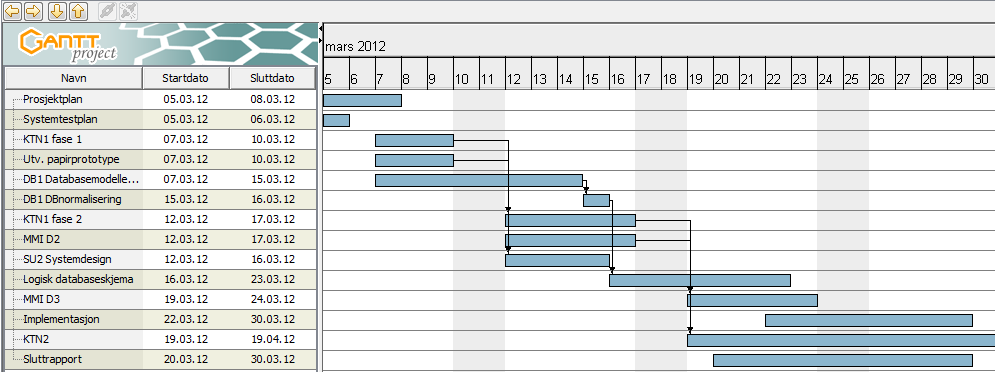
\includegraphics[scale=0.6]{{D:/dropbox/Private/FP/Gruppe34/FellesDoc/prosjektplan/gantt/gdgr34.png}}

\newpage

\part{Risk Analysis}

\begin{tabular}{|p{3cm}|p{2cm}|p{2cm}|p{4cm}|p{4cm}|}
\hline
Risk & Probability & Degree of severity & Consequences & Retirement plan \\ 
\hline
Illness/Absence caused by external factors & Moderate & Serious & Affected
individual is unable to complete their tasks & Participant's tasks must be
carried out by other participans \\ \hline
Late discovery of errors & High & Tolerable & Development slows down or halts
& Backtrack to the error's origin and correct affected areas \\ \hline
A task takes longer than expected & Moderate & Tolerable & Results in more
work than expected and possibly delayed progress & Alter the project plan,
distribute tasks to participants \\ \hline
Technical difficulties & Low & Serious & Planned solution is possibly
invalidated & Fix the technical issue or use another solution \\ \hline
The project is halted due to lack of knowledge & Low & Tolerable & 
Participant does not have the required knowledge to complete a task & 
Attempt to learn from team members, read up on subject material \\ \hline
Loss of group members & Low & Critical & Activities are left without
supervisor & Divide tasks amongst remaining participants \\ \hline
Internal disagreements & Low & Tolerable & Time is spent on discussions
rather than development & Maintain democracy and motivational levels \\ 
\hline
Change in specifications & Low & Tolerable & Both planned and implemented
solutions are invalidated & Discuss changes with student/teaching assistant
\\ \hline
\end{tabular}

\bigskip

\end{document}
